\documentclass[12pt]{article}
\usepackage{fullpage,graphicx,psfrag,amsmath,amsfonts,verbatim}
\usepackage[small,bf]{caption}

\input defs.tex

\bibliographystyle{alpha}

\title{Assignment 3 CME 241}
\author{Taylor Howell}

\begin{document}
\maketitle

\paragraph{1. Bellman Policy Equations (discrete policy)}
$$V^{\pi_D} = \mathcal{R}^{\pi_D}(s) + \gamma \sum\limits_{s' \in \mathcal{N}} \mathcal{P}^{\pi_D}(s, s') \cdot V^{\pi_D}(s')$$

$$Q^{\pi_D}(s,a) = \mathcal{R}^{\pi_D}(s, a) + \gamma \sum\limits_{s' \in \mathcal{N}} \mathcal{P}^{\pi_D}(s, s') \cdot Q^{\pi_D}(s', a')$$

$$Q^{\pi_D}(s,a) = \mathcal{R}^{\pi_D}(s, a) + \gamma \sum\limits_{s' \in \mathcal{N}} \mathcal{P}^{\pi_D}(s, s') \cdot V^{\pi_D}(s')$$

$$V^{\pi_D}(s) = \mathcal{R}^{\pi_D}(s) + \gamma \sum\limits_{s' \in \mathcal{N}} \mathcal{P}^{\pi_D}(s, s') \cdot Q^{\pi_D}(s',\pi_D(s'))$$

%\begin{figure}
%	\centering
%	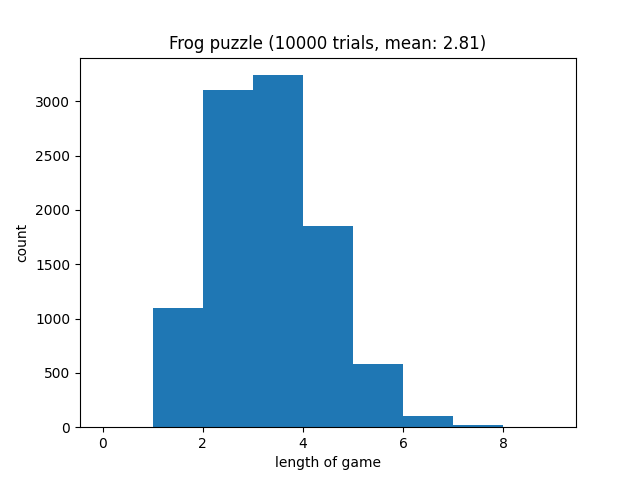
\includegraphics[width=.5\textwidth]{frog_puzzle_histogram.png}
%	\caption{Histogram showing the number of transitions to complete ``frog puzzle" for 10000 trials.}
%	\label{frog_puzzle}
%\end{figure}

\end{document}
